

\begin{figure}[ht]
  \centering

  \tikzstyle{smallsquare}=[
    draw,
    line width=1pt,
    minimum height=0.25in,
    minimum width=0.25in,
  ]

  \tikzstyle{dep}=[
    -latex,
    ultra thick,
  ]

  \begin{subfigure}[b]{0.3\textwidth}
    \centering
    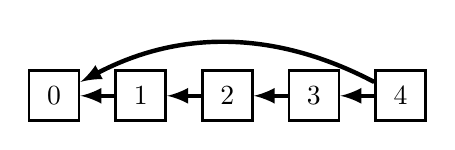
\begin{tikzpicture}[xscale=1.1]
      \foreach \i [count=\x] in {0, 1, 2, 3, 4} {%
        \node[smallsquare] (\i) at (\x, 0) {$\i$};
      }
      \draw[dep] (1) to (0);
      \draw[dep] (2) to (1);
      \draw[dep] (3) to (2);
      \draw[dep, bend right] (4) to (0);
      \draw[dep] (4) to (3);
    \end{tikzpicture}
    \caption{$G_1$}\figlabel{DeadlockBPaxosExampleG1}
  \end{subfigure}
  \hspace{1in}%
  \begin{subfigure}[b]{0.3\textwidth}
    \centering
    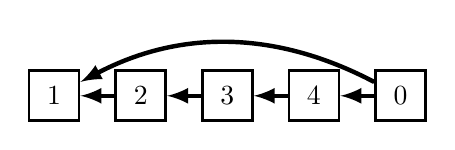
\begin{tikzpicture}[xscale=1.1]
      \foreach \i [count=\x] in {1, 2, 3, 4, 0} {%
        \node[smallsquare] (\i) at (\x, 0) {$\i$};
      }
      \draw[dep, bend right] (0) to (1);
      \draw[dep] (0) to (4);
      \draw[dep] (2) to (1);
      \draw[dep] (3) to (2);
      \draw[dep] (4) to (3);
    \end{tikzpicture}
    \caption{$G_2$}\figlabel{DeadlockBPaxosExampleG2}
  \end{subfigure}

  \vspace{0.2in}

  \begin{subfigure}[b]{0.3\textwidth}
    \centering
    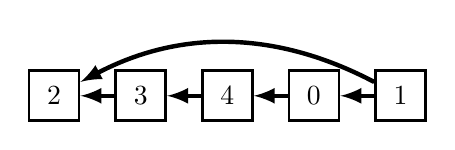
\begin{tikzpicture}[xscale=1.1]
      \foreach \i [count=\x] in {2, 3, 4, 0, 1} {%
        \node[smallsquare] (\i) at (\x, 0) {$\i$};
      }
      \draw[dep] (0) to (4);
      \draw[dep] (1) to (0);
      \draw[dep, bend right] (1) to (2);
      \draw[dep] (3) to (2);
      \draw[dep] (4) to (3);
    \end{tikzpicture}
    \caption{$G_3$}\figlabel{DeadlockBPaxosExampleG3}
  \end{subfigure}
  \hspace{1in}%
  \begin{subfigure}[b]{0.3\textwidth}
    \centering
    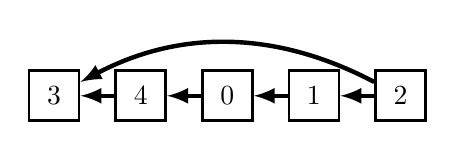
\begin{tikzpicture}[xscale=1.1]
      \foreach \i [count=\x] in {3, 4, 0, 1, 2} {%
        \node[smallsquare] (\i) at (\x, 0) {$\i$};
      }
      \draw[dep] (0) to (4);
      \draw[dep] (1) to (0);
      \draw[dep] (2) to (1);
      \draw[dep, bend right] (2) to (3);
      \draw[dep] (4) to (3);
    \end{tikzpicture}
    \caption{$G_4$}\figlabel{DeadlockBPaxosExampleG4}
  \end{subfigure}

  \vspace{0.2in}

  \begin{subfigure}[b]{0.3\textwidth}
    \centering
    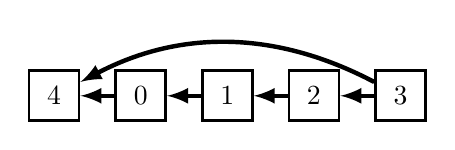
\begin{tikzpicture}[xscale=1.1]
      \foreach \i [count=\x] in {4, 0, 1, 2, 3} {%
        \node[smallsquare] (\i) at (\x, 0) {$\i$};
      }
      \draw[dep] (0) to (4);
      \draw[dep] (1) to (0);
      \draw[dep] (2) to (1);
      \draw[dep] (3) to (2);
      \draw[dep, bend right] (3) to (4);
    \end{tikzpicture}
    \caption{$G_5$}\figlabel{DeadlockBPaxosExampleG5}
  \end{subfigure}

  \caption{A Deadlock BPaxos deadlock}%
  \figlabel{DeadlockBPaxosExample}
\end{figure}
